%\documentclass{article}
%\usepackage{tikz}
%\usepackage{SIUnits}

%\begin{document}

\begin{figure}[tb]
	\centering
	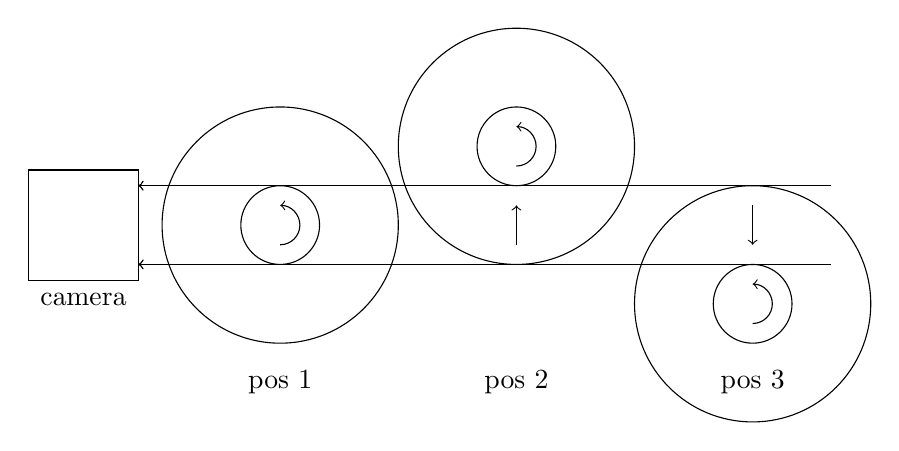
\begin{tikzpicture}
		%drawing grid
		% \draw[color=gray] (0,0) grid (8,1);
		%camera
		\draw (-.2,-.2) rectangle (1.2,1.2);
		\draw (.5,-.25) node [below] {camera};
		%position 1
			% beam
			\draw[<-] (1.2,0) -- (10,0);
			\draw[<-] (1.2,1) -- (10,1);
			%sample
			\draw (3,0.5) circle (.5);
			\draw (3,0.5) circle (1.5);
			\draw (3,-1.5) node {pos 1};
			% movement
			%\draw[->]  (3,1.25) -- (3,1.75);
			%\draw[->]  (3,-.25) -- (3,-.75);
			%sample rotation
			\draw[->] (3,0.25) arc (-90:90:.25);
		%position 2
			% sample
			\draw (6,1.5) circle (.5);
			\draw (6,1.5) circle (1.5);
			\draw (6,-1.5) node {pos 2};
			% movement
			\draw[->]  (6,.25) -- (6,.75);
			%sample rotation
			\draw[->] (6,1.25) arc (-90:90:.25);
		% position 3
			% sample	
			\draw (9,-.5) circle (.5);
			\draw (9,-.5) circle (1.5);
			\draw (9,-1.5) node {pos 3};
			% movement
			\draw[<-]  (9,.25) -- (9,.75);
			%sample rotation
			\draw[->] (9,-.75) arc (-90:90:.25);
		% beam
			\draw[<-] (1.2,0) -- (8,0);
			\draw[<-] (1.2,1) -- (8,1);
				% labels
		%\draw (2.5,1.25) node [above] {beam};
		%\draw (6.5,1.25) node [above] {beam};
		%\draw (4.5,-1) node [below] {sample};
	\end{tikzpicture}
	\caption{Covering the FOV -- three scans $\rightarrow$ sample has to move, explain that we still only do \unit{180}{\degree} scans!}
	\label{fig:covering-three scans}
\end{figure}

%\end{document}
